\section{\textcolor{blue}{Preliminares: ENO}}

\begin{frame}{Preliminares: ¿Qué es un Espacio Normado Ordenado?}
	\begin{columns}
		\column{.45\textwidth}
		$-$\textbf{Definición: \cite{cone2007} }
		\begin{block}{}
			Sea $ (X, || \cdot || ) $ un espacio normado y  $ X_{+} \subset  X$ cerrado no vacío.\\ Se dice que $ X_{+} $ es un \textbf{cono}\\ si $ x, \ y \in X_{+} $, $\lambda \geq 0$ cumplen:
			\begin{itemize}
				%\item $P$ es cerrado en $X$.
				\item  $x + y \in X_{+}$.
				\item  $\lambda x \in X_{+}$.
				\item  $-x, \ x \in X_{+}$ implica $x = \bar{0} $.
				%\item $P$ es cerrado.
			\end{itemize}
			
		\end{block}
		A  $(X, || \cdot | | , X_{+}  )$ se le llama \textbf{espacio normado ordenado}.\\
		
		\column{.45\textwidth}
	
			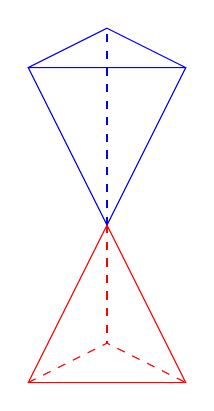
\begin{tikzpicture}
			%Tetraedro azul
			\draw[color=blue] (0,-1) -- (-1,1) -- (1,1) -- (0,-1); 
			\draw[color=blue] (-1,1) -- (0,1.5) -- (1,1);
			\draw[ dashed, color=blue]  (0,-1) -- (0,1.5);
			%Tetraedro Rojo
			\draw[color=red] (0,-1) -- (-1,-3) -- (1,-3) -- (0,-1); 
			\draw[ dashed, color=red] (-1,-3) -- (0,-2.5) -- (1,-3);
			\draw[ dashed, color=red]  (0,-1) -- (0,-2.5);
		\end{tikzpicture}
		\textcolor{blue}{$ X_{+} + \lambda X_{+} \subset X_{+} $.}\\ \textcolor{blue}{$X_{+} $} $\cap$  \textcolor{red}{$(- x_{+} )$} $= \{ \bar{0} \}$.
	\end{columns} 
\end{frame}

%%%%%%%%%%%%%%%%%%%%%%%%%%%%%%%%%%%%%%%%%%%%%%%%%%%%%%%%%%%%%%%%%%%%%%%%%%%%%%%%%%%%%%%%%%%%%%%%%%%%%%%%%%%%%%%%%%%%%%%%%%%%%%%%%%%%%%%%%%%%%%%%%%%%%%%%%%%%%%%%%%%%%%%%%%%%%%%%%%%%%%%%%%%%%%%%%%%%%%%%%%%%%%%%%%%%%%%%%%%%%%%%%%%%%%%%%%%%%%%%%%%%%%%%%%%%%%%%%%%%%%%%%%%%%%%%%%%%%%%%%%%%%%%%%%%%%%%%%%%%%%%%%%%%%%%%%%%%%%%%%%%%%%%%%%%%%%%%%%%%%%%%%%%%%%%%%%%%%%%%%%%%%%%%%%%%


\begin{frame}{}
	\begin{block}{Teorema}
			Sean $(X, || \cdot || , X_{+} )$ un ENO, $ a,b,c \in X$ y $ \lambda \geq 0$. Entonces la relación  $``\leq "$ en $X$   definida como $a \leq b$ si $b-a \in X_{+}$  cumple que
		\begin{enumerate}[(1)]
			\item $a \leq a$, 
			\item Si $a \leq b$ y $b \leq a$, entonces $ a=b $, 
			\item Si $a \leq b$ y $b \leq c$, entonces $a \leq c$, 
			\item Si $a \leq b$, entonces $a+c \leq b+c$, 
			\item $ a \leq b$, entonces $\lambda a \leq \lambda b $.
		\end{enumerate}
	\end{block}
Nota:	$ a < b $, si $ a \leq b  $ y  $ a \neq b . $ 
\end{frame}
	%%%%%%%%%%%%%%%%%%%%%%%%%%%%%%%%%%%%%%%%%%%%%%%%%%%%%%%%%%%%%%%%%%%%%%%%%%%%%%%%%%%%%%%%%%%%%%%%%%%%%%%%%%%%%%%%%%%%%%%%%%%%%%%%%%%%%%%%%%%%%%%%%%%%%%%%%%%%%%%%%%%%%%%%%%%%%%%%%%%%%%%%%%%%%%%%%%%%%%%%%%%%%%%%%%%%%%%%%%%%%%%%%%%%%%%%%%%%%%%%%%%%%%%%%%%%%%%%%%%%%%%%%%%%%%%%%%%%%%%%%%%%%%%%%%%%%%%%%%%%
	\begin{frame}{}
		$-$\textbf{Definición:} 
		\begin{block}{}
		    	Sean $(X,|| \cdot || , X_{+} ) $ un ENO y $ a, b \in X_{+} $ con $ a \leq b  $. 
		\begin{itemize}
			\item $[a , b ] = \left\lbrace  x \in X : a \leq x \leq b \right\rbrace  $ se llama  \textbf{intervalo ordenado cerrado} de $(X,\leq)$.
	 	\item $[a, \infty ) = \left\lbrace  x \in X : a \leq x  \right\rbrace  $  se llama  \textbf{intervalo ordenado infinito  semicerrado por la izquierda } de $(X,\leq)$.\\
    Análogamente se define $( - \infty, a ] $ el \textbf{intervalo ordenado infinito  semicerrado por la derecha}.
		\end{itemize}
		\end{block}
		
	\end{frame}

